\documentclass[preprint, hmargin=1in, vmargin=1in]{aastex62}
%%%%%%begin preamble
%\usepackage[hmargin=1in, vmargin=1in]{geometry} % Margins
\usepackage{hyperref}
\usepackage{url}
\usepackage{natbib}
\setlength{\bibsep}{0pt plus 0.3ex}
\usepackage{graphicx}
\usepackage{amsmath}
\usepackage{amsfonts}
\usepackage{amssymb}
%\usepackage{import}
\usepackage{wrapfig}

\usepackage{color}
\hypersetup{
  colorlinks   = true,
  %citecolor    = blue
  citecolor    = gray
  % gray is not being found!?!
  % gray is found if pdfpages is used... crap.
  %citecolor    = grey
  %citecolor    = Gray
}

%% headers
\usepackage{fancyhdr}
\pagestyle{fancy}
\fancyhf{} % sets both header and footer to nothing
\lhead{Evan Anders -- Research Proposal}
\rhead{NASA Hubble Fellowship Program}
\cfoot{\footnotesize{\thepage}}
%\pagestyle{empty}
%\pagenumbering{gobble}
%\renewcommand*{\thefootnote}{\fnsymbol{footnote}}

\renewcommand{\vec}{\ensuremath{\boldsymbol}}
\newcommand{\dedalus}{\href{http://dedalus-project.org}{Dedalus}}
\newcommand{\del}{\ensuremath{\vec{\nabla}}}
\newcommand{\scrS}{\ensuremath{\mathcal{S}}}

\newcommand{\prf}{Physical Review Fluids}

%\newcommand{\nosection}[1]{%
%  \refstepcounter{section}%
%  \addcontentsline{toc}{section}{\protect\numberline{\thesection}#1}%
%  \markright{#1}}
%\newcommand{\nosubsection}[1]{%
%  \refstepcounter{subsection}%
%  \addcontentsline{toc}{subsection}{\protect\numberline{\thesubsection}#1}%
%  \markright{#1}}

%\usepackage{atbegshi}
%%%%%%end preamble


\begin{document}
\begin{center}
\Large{Convective Conundrums in the Asteroseismic Age:\\\vspace{-6pt}The interplay of rotation and magnetism in stellar convection} \\
\large{Evan H. Anders }
\end{center}
\vspace{-0.2cm}



Main sequence stars of masses similar to the Sun rely on vigorous near-surface convective regions to transport their stellar luminosity.
These convecting regions are highly stratified (14 density scale heights in the Sun), and the convective motions generate sound waves which refract due to stratification as they propagate into the stellar interior.
Helioseismology and asteroseismology measure the surface signatures of these acoustic waves---and gravity modes when available---to examine the interior of the Sun and other stars.
These measurements enable the precise determination of mass and radius of other stars, and have revealed the interior structure and mean flows, like differential rotation, inside the Sun \citep{huber&all2019, christensen-dalsgaard2002}.

Interpretation of asteroseismic and helioseismic data relies on one-dimensional (1D) stellar structure models. 
State-of-the-art codes like MESA \citep{paxton&all2011} which generate 1D stellar structure profiles have many deficiencies \citep{buldgen2019}, including their reliance on parameterizations of convection like mixing length theory \citep[MLT,][]{bohm-vitense1958}.
Parameterizations like MLT assume that convective flows whose length scales are proportional to the local density scale height are driven throughout the full depth of the convective zone.
This theory thus predicts that small convective elements driven near the stellar surface---like the ``granules'' we see on the Sun's surface---should exist on top of large-scale ``giant cells'' driven in the deep convection zone.
Unfortunately, modern helioseismic observations and direct measurements of flows on the Sun's surface have not detected giant cells \citep{hanasoge&all2015}.
The absence of these flows has called into question our most fundamental understanding of the nature of convection in stars, a problem widely referred to as the ``Solar Convective Conundrum.''
Improving our understanding of convection, and thus improving stellar structure models is critical to improving asteroseismic observations.
With NASA's TESS mission currently underway and supplying more than $10^4$ asteroseismic target stars in its nominal mission, and with other missions such as WFIRST increasing the number of asteroseismic target stars to $10^6$ \citep{huber&all2019}, we must sort out the convective conundrum.

My research aims to  help solve this Convective Conundrum by gaining a better understanding of convection in the highly stratified, rotating, magnetized context of stellar convection.
Parameterizations like MLT generally neglect stellar rotation and magnetism, but modern asteroseismic observations have detected latitudinal differential rotation in stars \citep{benomar&all2018} and shown that the structure of stellar magnetic fields affects asteroseismic measurements \citep{santos&all2018}.
As a Hubble fellow, I will conduct a series of studies which will span from the smallest to the largest scales present in stellar convection to better understand the importance of rotation and magnetism on stellar convection and structure.
I will build up understanding in detailed, small-scale studies to later inform the production and interpretation of large-scale global studies.
While I draw my inspiration from problems facing the solar and stellar community, similar flow processes may be important in the atmospheres and cores of planets like Jupiter and the Earth. 

\vspace{-55pt}
\section{Numerical Explorations of the Entropy Rain Hypothesis}
\paragraph{The Entropy Rain hypothesis}
In incompressible convection, velocity and temperature fields are symmetrical in upflows and downflows; atmospheric density stratification breaks this symmetry.
Stratified convection exhibits upwellings that are slow, weak, and wide in balance with downflows which are intense, fast, and narrow.
It has been hypothesized that downflows may be so powerful in the context of solar-like convection that they alone transport the stellar luminosity.
These downflows would exist alongside mass-conserving upflows which exhibit negligible energy transport.
This ``entropy rain'' hypothesis, first suggested by \citet{spruit1997}, is gaining traction, and could explain the absence of giant cells in observations \citep{hanasoge&all2015}.
Recent simulations of solar-like convection suggest that surface-driven downflows can indeed transport most of the stellar luminosity \citep{kapyla&all2017}, and recent theoretical work showed that such a concept could be included into 1D parameterizations \citep{brandenburg2016}.
A schematic of the entropy rain picture is shown in Fig.~\ref{fig:tri_panel}a.


\paragraph{Convection at the smallest scales: individual downflows} 
Modern results suggest that stellar downflows deserve more careful study.
It is possible these downflows turbulently break up into distinct pieces as they fall and these individual downflow pieces can be well modeled as ``thermals.''
Thermals are regions of cold fluid which accelerate due to buoyancy forces and shape themselves into vortex rings; evolved thermals are visualized in Fig. \ref{fig:tri_panel}b.
Thermals are also observed and studied in the Earth's atmosphere \citep{lecoanet&jeevanjee2019}.

\begin{figure*}[t]
    \includegraphics[width=\textwidth]{./figs/tri_panel.png}
    \caption{ (a) A schematic of the interior of solar-like stars under the entropy rain hypothesis.
	Rather than large convective rolls (giant cells) occupying the bulk of the stellar convection zone, cold droplets of fluid carry the stellar luminosity below a small convective surface layer.
	The first two experiments proposed here are boxed and labeled (``Thermals'' and ``RCB''), and the third experiment proposed here would contain the full spherical volume of the star.
	(b) A 3D visualization of entropy perturbations within the downward-propagating reference frame of a turbulent thermal, which may be the dynamical form of entropy rain.
	The first experiment proposed here would determine how rotation and magnetism affect the propagation of these structures.
	(c) A schematic of the radiative-convective boundary (RCB), where downflows impinge upon a stable layer and excite gravity waves within that layer.
	The second experiment proposed here would study how effectively these entropy rain downflows pump angular momentum and magnetic fields across the RCB.
	\label{fig:tri_panel} }
\end{figure*}


During my PhD, I gained proficiency in using the open-source Dedalus \citep{burns&all2019} code to study questions about stellar convection at various scales.
I used Dedalus to study thermals-as-downflows and learned how atmospheric stratification affects the propagation of these downflows \citep{andersLB2019}.
I surprisingly found that these downflows carry enough energy to feasibly transport the stellar luminosity, giving credence to the entropy rain hypothesis.
However, this work neglected turbulence, magnetism, and rotation, which are key ingredients in stellar convection.

As a Hubble fellow, I will build upon this study from my thesis work to understand if entropy rain is feasible by including solar-like complications.
Rotation, magnetism, and turbulence could all have filtering effects on downflows, preventing their successful transit of the stellar convection zone in certain regimes.
I will determine whether strong magnetic fields and global rotation can ``evaporate'' entropy rain.
While \citet{lecoanet&jeevanjee2019} found that turbulence had little effect on the evolution of thermals in unstratified atmospheres, the compressional effects of atmospheric stratification could change this outcome, and I will explore this possibility.
Understanding if the inclusion of these realistic effects prevents downflows from crossing the stellar convection zone will help determine the validity of the entropy rain hypothesis.
As in \citet{andersLB2019}, these studies will include both analytical and numerical analyses.

\paragraph{Convection at the mesoscale: interactions at the radiative-convective boundary}
In Sun-like stars, the turbulent convection zone lies above a stably stratified ``radiative zone'' where radiation effectively carries the stellar luminosity.
In the Sun, the radiative-convective boundary (RCB) is characterized by a transition from moderate instability to strong stability.
The solar RCB furthermore coincides with a region of intense shear in the Sun's radial velocity profile called the tachocline, and it is thought that these shear interactions are a crucial driver of the Sun's magnetic dynamo.
In the entropy rain picture, constraining the pumping of angular momentum and magnetism into the RCB is crucial to figuring out how the dynamos and differential rotation profiles of stars are driven.
Measurements suggest that the Sun's RCB is thin \citep{basu1997}, but many modern simulations produce RCBs which are up to an order of magnitude thicker than the solar one \citep{hotta2017}.
This suggests that many simulations are studying angular momentum and magnetic field pumping mechanisms in the wrong regime of ``stiffness'' of the RCB \citep{couston&all2017}.

%\begin{figure*}[t!]
%    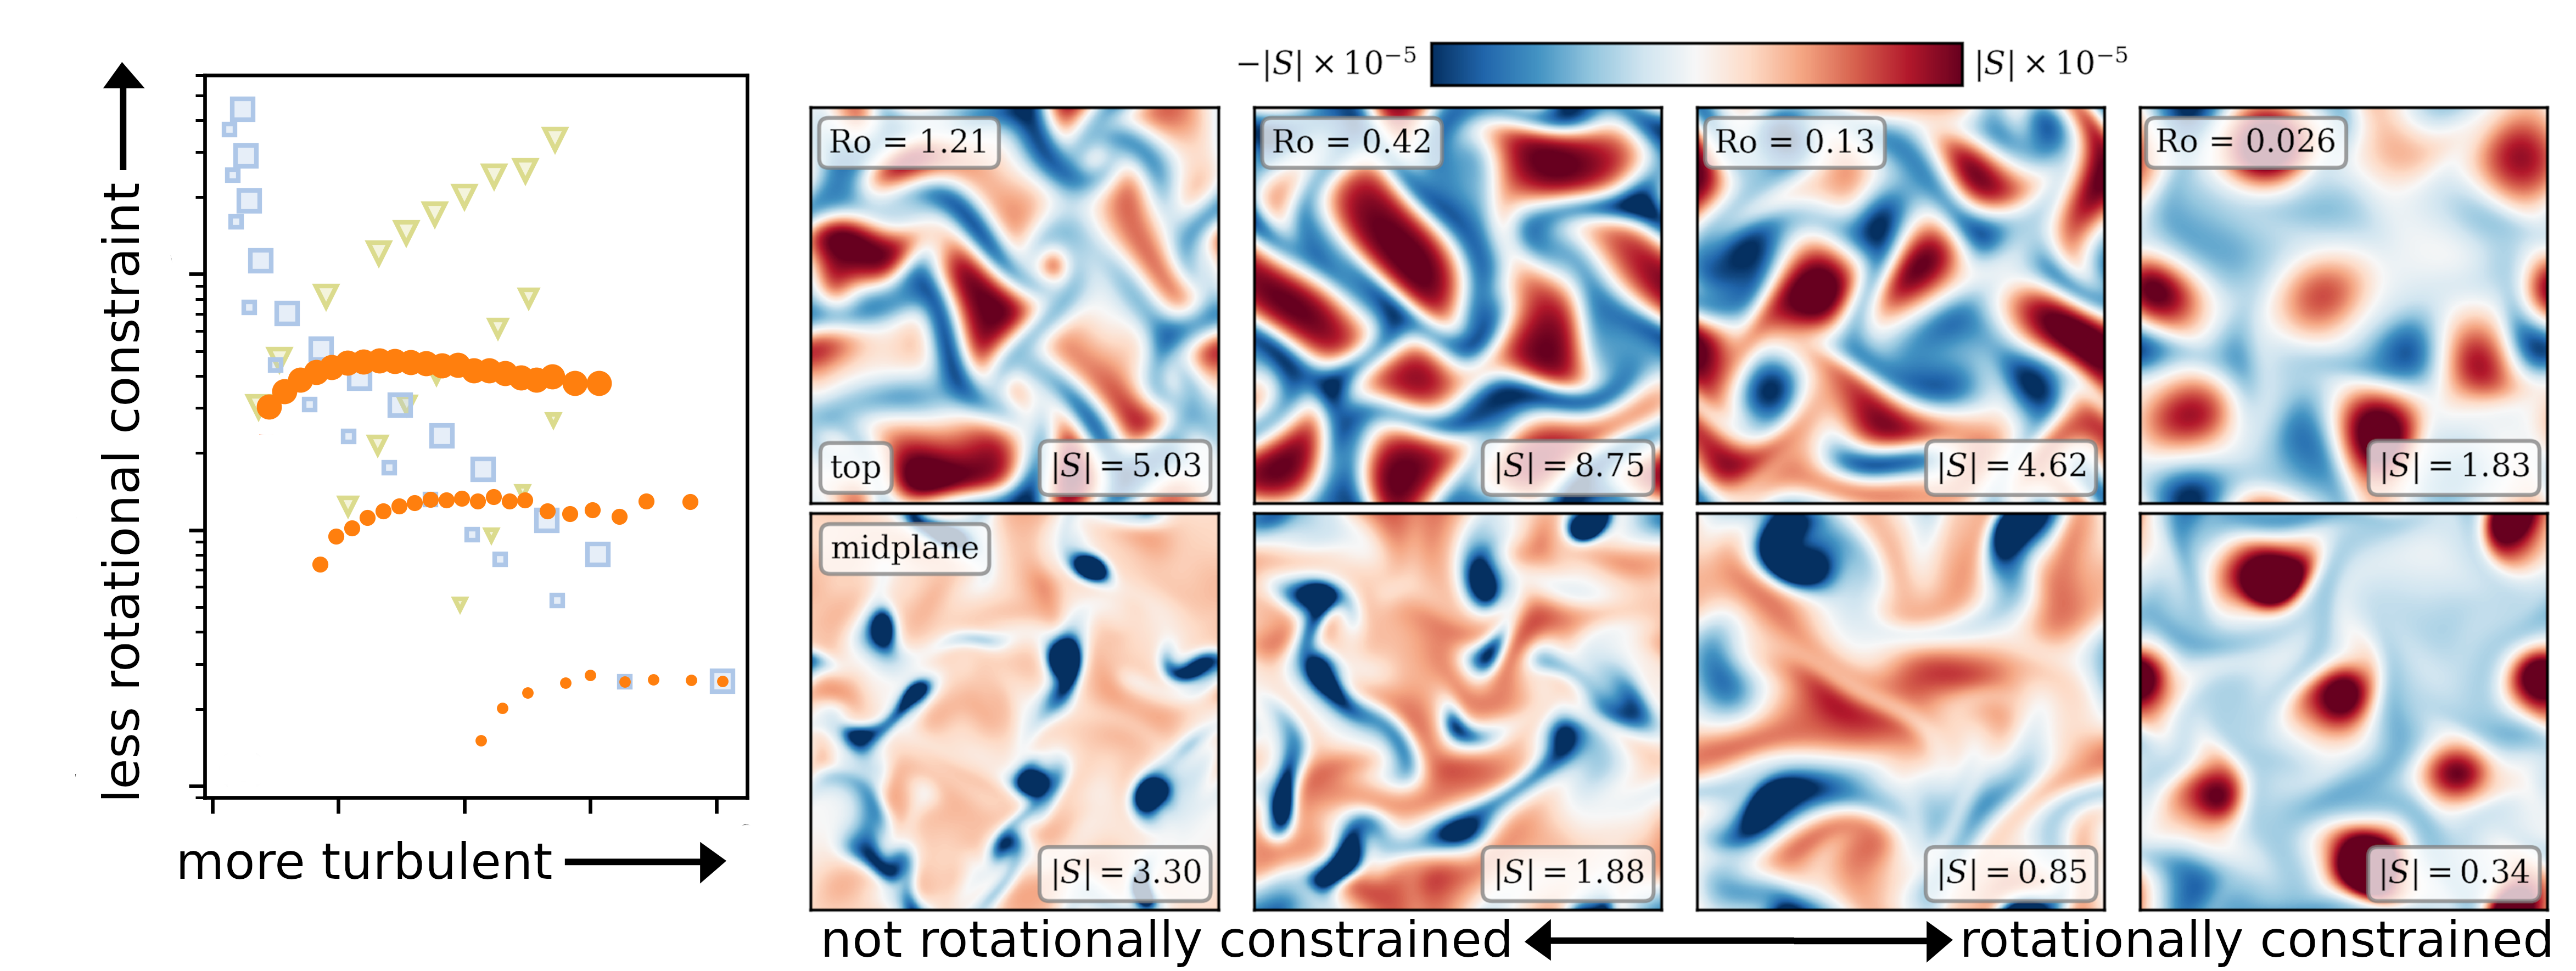
\includegraphics[width=\textwidth]{./figs/rossby_plot.png}
%    \caption{(left, Fig 1b of \citet{anders&all2019}) The importance of rotation is difficult to predict as turbulence is increased in convective simulations.
%	Rotational influence varies greatly along traditional paths through parameter space (green triangles and blue squares).
%	We have discovered a new parameter (orange circles) that allows rotational influence to be specified \emph{a priori}.
%	(right eight panels, Fig. 2 of \citet{anders&all2019}) As convective flows become increasingly rotationally constrained (from left to right), their morphology changes and they vary less as a function of height (top compared to bottom).
%	It is crucial to simulate solar convection under the same rotational influence as the real Sun to ensure that flow topologies and interactions are an accurate model.
%	\label{fig:rossby_plot} }
%\end{figure*}
%
%In creating simulations of stellar convection, it is important to strive to produce flows which feel the same influence of rotation and magnetism as those in the star being studied.
%Simulations which include global rotation can be run in a regime where flows are heavily affected by Coriolis forces or one where Coriolis forces are weak.
%A ``critical'' rotation frequency, $\Omega_\text{c}$, separates these two regimes, but determining $\Omega_\text{c}$ is often not straightforward.
%During my PhD, I found a method for determining $\Omega_\text{c}$ so that the importance of rotation could be specified in simulation initial conditions \citep[see left panel of Fig. \ref{fig:rossby_plot} and][]{anders&all2019}.
%Flows look very different depending on whether you simulate above, below, or near $\Omega_\text{c}$ (right panels of Fig.~\ref{fig:rossby_plot}), and it is crucial to simulate in the same regime as the Sun.
%In magnetized systems, there is an analagous critical magnetic field, but to date no study has determined how to determine this field \emph{a priori}.

As a Hubble fellow, I will study how an ensemble of downflows interacts with a solar-like RCB in the presence of solar-like rotation and magnetism.
To do this, I will study mesoscale simulations of time-evolving convective simulations where unstable convection zones overlay stable radiative interiors, extending the work I performed in \citep{anders&brown2017, anders&all2019} in setups similar to those in \citep{kapyla&all2017}. 
These simulations will be primarily conducted in the regimes where the previous downflow-only simulations determined that downflows are not filtered out by rotation and magnetism.
If downflows are capable of effectively pumping magnetism and angular momentum into the RCB, then it is probable that the popular picture of the RCB and tachocline as a driver of global magnetic field.
If downflows cannot carry these quantities into the RCB, then magnetic fields are likely generated by another process.
In addition to helping determine where stellar dynamos are driven, these studies will help determine the stellar rotation rates and luminosities in which downflows can effectively establish solar-like differential rotation profiles through RCB interactions.

\section{Global scale convection: dynamics in relaxed atmospheres}
MLT's deficiencies have led some researchers to seek out ways to couple 1D models with fully convective, three-dimensional (3D) global simulations.
Such a coupling has recently been performed with some success \citep{jorgensen&weiss2019}, but the 3D simulations utilized were localized in a very thin layer near the stellar surface.
Furthermore, \citet{jorgensen&weiss2019} coupled previously computed 3D simulations with 1D models, rather than coupling the two at runtime, largely because 3D simulations are costly.
Some of these costs are unavoidable: highly resolved, turbulent simulations necessarily take small timesteps, and therefore simulation times are very long.
Thin, near-surface simulations such as those used by \citet{jorgensen&weiss2019} examine a regime where the convective overturn timescale is very similar to the local Kelvin-Helmoltz (KH) timescale of atmospheric equilibration.
In studies of deep convection these timescales become disparate, and many overturn timescales pass during one KH timescale.
Thus, much of the expense of simulations which include deep convection is often time ``wasted'' waiting for the atmospheric structure and mean flows to converge to an equilibrium state.
This expense can be minimized through the use of clever numerical techniques.

During my PhD, I created and verified an ``accelerated evolution'' tool which skips the long KH timescale in convective simulations \citep{anders&all2018}.
This tool reached a relaxed, equilibrated state using an order of magnitude fewer computational resources than a simulation which timestepped through a full KH timescale, and results between the simulations differed by less than 1\%.

\begin{wrapfigure}{r}{0.3\textwidth}
	\begin{center}
	\vspace{-10pt}
    \includegraphics[width=0.28\textwidth]{./figs/mdwarf.png}
	\vspace{-16pt}
	\end{center}
    \caption{A volume rendering of a global dynamo simulation in Dedalus.
	Enstrophy, or the magnitude of vorticity, is shown in green.
	Red and blue lines denote the magnitude and direction of azimuthal magnetic field.
	\label{fig:mdwarf} }
\end{wrapfigure}


As a Hubble fellow, I will extend my accelerated evolution method to the evolution of thermodynamic and angular momentum profiles in global simulations.
Dedalus is capable of accurately simulating global domains which include the origin at $r = 0$ \citep{lecoanet&all2019}; a visualization of basic outputs from these simulations is shown in Fig.~\ref{fig:mdwarf}.
The large-scale structures seen in Fig.~\ref{fig:mdwarf} arise quickly, but the equilibration and saturation of these structures and other simulation measurements often takes KH timescales which cannot be feasibly simulated in turbulent regimes.
I will design a generalized public module which can accelerate mean profiles and flows in global simulations.
This module will read in statistical measures from unequilibrated convective simulations and output the properly equilibrated mean state.
Researchers simulating convection with Dedalus or other codes will be able to use this module to rapidly equilibrate simulations with state-of-the-art turbulent dynamics.
This tool will benefit numericists across diverse research fields, such as those who study general circulation models (GCMs) in the atmospheres of the Earth and exoplanets or modelers of dynamo processes in planetary cores and stellar atmospheres.
Once completed, I will use this tool in my own research to accelerate the evolution of highly turbulent, solar-like simulations to understand the nature of global flows and dynamos in an equilibrated simulation.


\section*{Relevance to NASA Astrophysics and Justification of Institute}
Improving models of stellar evolution is crucial to determining our cosmic origins and answering the question, \emph{``How did we get here?''}
Convective processes are important for stars of all masses and influence the determined radius or age of a star.
Asteroseismology can measure stellar masses and the radii of stars with exoplanets, and can be used to determine the properties of large stellar populations for uses in galactic archaeology.
Uncertainties in our convective models, which the Convective Conundrum have made clear, limit the accuracy of these techniques, and in doing so impede studies of exoplanets and galactic archaeology by missions like TESS, JWST, and WFIRST.
To understand how we got here, we need to understand stellar convection better to improve stellar evolution and stellar structure models.

Northwestern university, and specifically the Center for Interdisciplinary Exploration and Research in Astrophysics (CIERA), is the perfect location for me to carry out this proposed work.
Prof.~Daniel Lecoanet, who will be my primary advisor and collaborator, is a core developer of Dedalus.
His expertise using Dedalus and his past work on thermals \citep{lecoanet&jeevanjee2019, tarshish&all2018}, convection \citep{lecoanet&quataert2013, lecoanet&all2014}, convection-stable layer interactions \citep{lecoanet&all2016, couston&all2017}, rotating convection \citep{couston&all2019}, and global simulations \citep{lecoanet&all2019} will make him a valuable collaborator and advisor for the projects proposed here.
Furthermore, I have already published a paper on thermals in close collaboration with Prof.~Lecoanet \citep{andersLB2019}, so the small scale studies of thermals proposed here will be an excellent transition project into my postdoctoral studies on my arrival.
In addition to Prof.~Lecoanet, Prof.~Yoram Lithwick would be an excellent partner for collaboration due to his work on rotating convection \citep[e.g.,][]{BDLithwick2014}.
CIERA houses many experts in computational fluid dynamics beyond Profs.~Lecoanet \& Lithwick, such as Profs.~Sasha Tchekhovskoy \& Claude-Andre Faucher-Giguere.
I look forward to joining the astrophysical fluid dynamics group at CIERA where I will have many opportunities to discuss and develop new numerical techniques, strategies, and applications across astrophysics.


\bibliographystyle{yahapj}
\bibliography{biblio}
\end{document}
